\documentclass[aps,pra,showpacs,notitlepage,onecolumn,superscriptaddress,nofootinbib]{revtex4-1}
\usepackage[utf8]{inputenc}
\usepackage[tmargin=1in, bmargin=1.25in, lmargin=1.5in, rmargin=1.5in]{geometry}
\usepackage{amsmath, amssymb, amsthm}
\usepackage{graphicx}
\usepackage{xcolor}
\usepackage{enumitem}
\usepackage{datetime}
\usepackage{hyperref}
\usepackage{titlesec}
\usepackage{import}
\usepackage{mathtools}
\usepackage{thmtools,thm-restate}
\usepackage{comment}


% package for commutative diagrams
% \usepackage{tikz-cd}

%%%%%%%%%%%%%%%%%%%%%%%%%%%%%%%%%%%%%%%%%%%%%
\definecolor{crimson}{RGB}{186,0,44}
\definecolor{moss}{RGB}{0, 186, 111}
\newcommand{\pop}[1]{\textcolor{crimson}{#1}}
\newcommand{\zcom}[1]{\noindent\textcolor{crimson}{(Z): #1}}
\newcommand{\jcom}[1]{\noindent\textcolor{moss}{(J): #1}}
\newcommand{\wt}[1]{\widetilde{#1}}
\newcommand{\pqeq}{\succcurlyeq}
\newcommand{\pleq}{\preccurlyeq}
\newcommand{\hhrulefill}{\hspace{-1em} \hrulefill}

%%%%%%%%%%%%%%%%%%%%%%%%%%%%%%%%%%%%%%%%%%%%%
\hypersetup{
    colorlinks,
    linkcolor={crimson},
    citecolor={crimson},
    urlcolor={crimson}
}

\usepackage{qcircuit}

%%%%%%%%%%%%%%%%%%%%%%%%%%%%%%%%%%%%%%%%%%%%%
\theoremstyle{definition}
\newtheorem{definition}{Definition}[section]
\newtheorem{lemma}{Lemma}[section]
\newtheorem{theorem}{Theorem}[section]
\newtheorem{corollary}{Corollary}[theorem]
\newtheorem*{theorem*}{Theorem}
\newtheorem*{corollary*}{Corollary}
\newtheorem{remark}{Remark}[section]
\newtheorem{conjecture}{Conjecture}[section]
\newtheorem{example}{Example}[section]
\newtheorem{reminder}{Reminder}[section]
\newtheorem{problem}{Problem}[section]
\newtheorem{question}{Question}[section]
\newtheorem{answer}{Answer}[section]
\newtheorem{fact}{Fact}[section]
\newtheorem{claim}{Claim}[section]
\newtheorem{proposition}{Proposition}[section]

\usepackage{geometry}
\geometry{
  left=25mm,
  right=25mm,
  top=20mm,
}
\usepackage{mathtools}

%%%%%%%%%%%%%%%%%%%%%%%%%%%%%%%%%%%%%%%%%%%%%
\bibliographystyle{unsrt}

%%%%%%%%%%%%%%%%%%%%%%%%%%%%%%%%%%%%%%%%%%%%%
%%%%%%%%%%%%%%%%%%%%%%%%%%%%%%%%%%%%%%%%%%%%%
%%%%%%%%%%%%%%%%%%%%%%%%%%%%%%%%%%%%%%%%%%%%%
\begin{document}

\title{Discrete Riemann surfaces and the Ising model: notes}
\author{Jack Ceroni}
\email{jackceroni@gmail.com}

\date{\today}

\maketitle

\section{Introduction}

\noindent The goal of these notes is to summarize and explain in greater detail the ideas outlined in Christian Mercat's paper \emph{Discrete Riemann surfaces and the Ising model}.
My main goal is for these notes to be \emph{self-contained}, \emph{exhaustive}, and \emph{rigorous}. Ultimately, I want this to be a comprehensive deconstruction of a mathematical paper
which can stand alone, and be understood by individuals with basic background in differential geometry.

\section{Introducing the terminology of discrete surfaces}

\noindent We begin by letting $\Sigma$ be an oriented surface without boundary. In these notes, we will in addition assume that $\Sigma$ is a smooth manifold (it has a smooth structure which
has smooth transition maps).

\begin{comment}
\begin{definition}[Orientation from the tangent bundle]
  The most common definition for the orientation of a smooth manifold, and the one most likely known by the reader, is the following.
  Given a manifold $M$, an \emph{oriented atlas} of $M$ is an atlas of open neighbourhoods and associated coordinate charts, $(U_{\alpha}, \varphi_{\alpha})_{\alpha \in I}$
  such that each transition map $\varphi_{\alpha} \circ \varphi_{\beta}^{-1}$ (which is assumed to be $C^{\infty}$ as $M$ is smooth) has positive Jacobian determinant everywhere.
  An \emph{orientation} on a manifold is a smooth structure (a maximal smooth atlas) which is oriented.
\end{definition}
\end{comment}

\subsection{Introducing cell complexes}

\noindent We now come to the first set of definitions. In particular, we develop a means of placing a discrete, lattice-like structure on an otherwise continuous surface,
in such a way that the underlying geometry of the surface is repsected.

\begin{definition}[Cellular decomposition]
  Given $\Sigma$ as defined above (an oriented surface without boundary), a \emph{cellular decomposition} $\Gamma$ of $\Sigma$ is a partition of $\Sigma$ into disjoint connected
  sets (which we call cells) of three different types:
  \begin{itemize}
  \item A discrete set of points. We call these the \emph{vertices} of $\Gamma$, and denote them by $\Gamma_0$
  \item A collection of non-intersecting sets of the form $\gamma((0, 1))$, where $\gamma : [0, 1] \rightarrow \Sigma$ is a bijective path such that $\gamma(0)$ and $\gamma(1)$, the endpoints of the path, are contained
    in $\Gamma_0$. We will assume that any such $\gamma$ is also smooth, in the sense that each $\varphi_{\alpha} \circ \gamma$ is smooth for $x \in \gamma((0, 1)) \cap U_{\alpha}$, where $(U_{\alpha}, \varphi_{\alpha})$ is a coordinate chart
    of the smooth structure on $\Sigma$. We call these the \emph{edges} of $\Gamma$ and denote them by $\Gamma_1$.
  \item A collection of topological discs of the form $B$ (in other words, an embedding of an open ball $B^2$ in $\Sigma$)
    such that $\partial B$ can be written as a finite union of elements of $\Gamma_0$ and $\Gamma_1$ (nodes and edges). We call these the \emph{faces} of $\Gamma$, and denote them by $\Gamma_2$.
  \end{itemize}
  A cellular decomposition is said to be \emph{locally finite} if every compact subset $C$ of $\Sigma$ intersects only a finite number of elements of $\Gamma$.
\end{definition}

\begin{center}
  \begin{figure}
    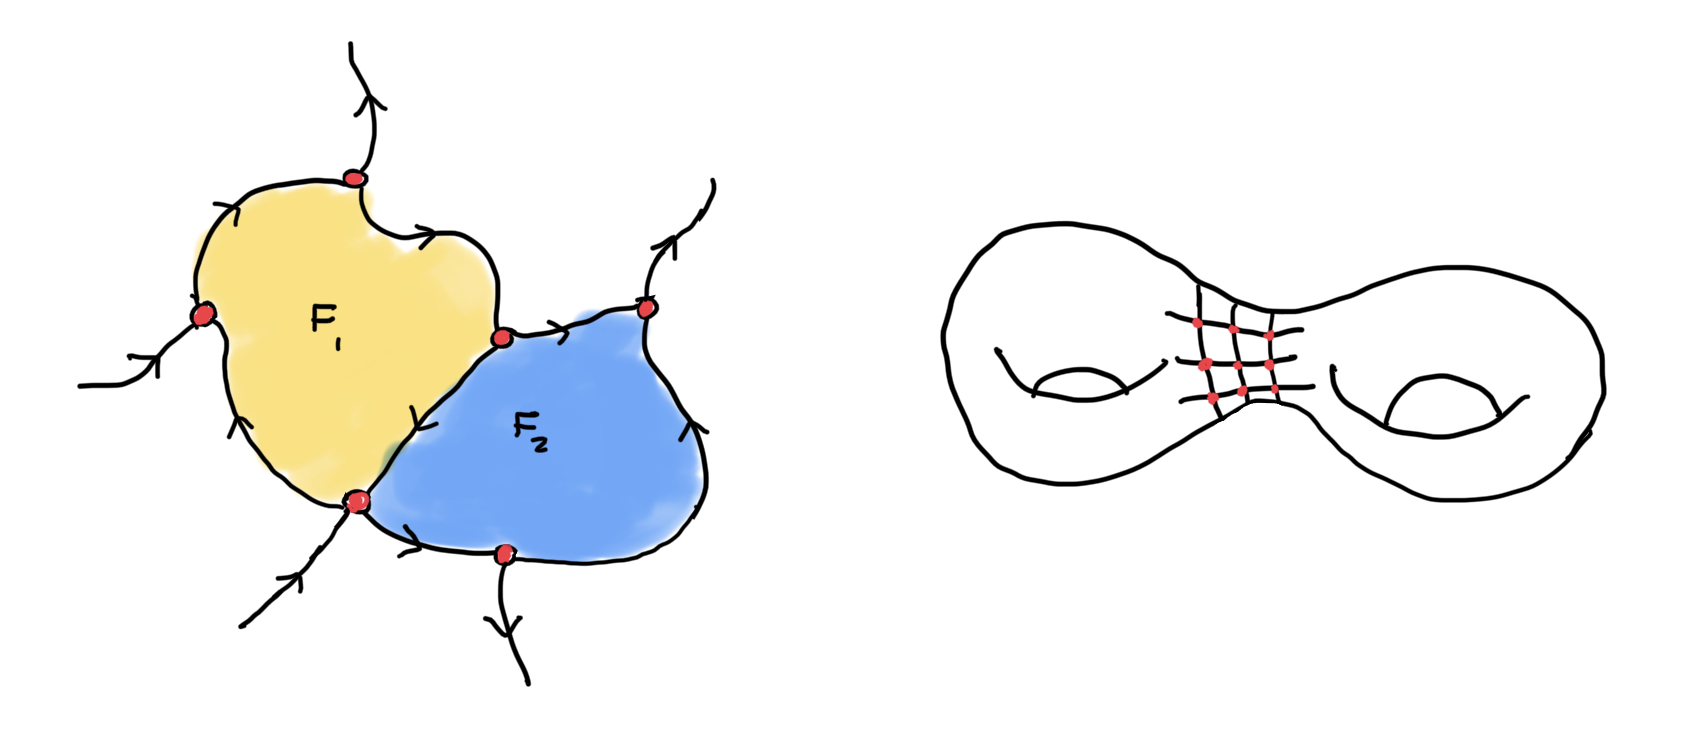
\includegraphics[width=400pt]{./assets/mercat1.jpeg}
    \caption{The left image depicts two faces $F_1$ and $F_2$ and their bounding, oriented edges (and vertices) of some cellular decomposition $\Gamma$. The right picture shows
    some of the cells of a cellular decomposition $\Gamma$ of a genus-$2$ surface $\Sigma$.}
    \end{figure}
  \end{center}

\begin{remark}[Parameterizing $\Gamma$]
  Note that the vertices, edges and faces of a cellular decomposition $\Gamma$ are all images of a $0$-ball (a point), $1$-ball (the interval $(0, 1)$), and $2$-ball (the set $\{x \in \mathbb{R}^2 \ | \ |x| < 1\}$), respectively,
  with respect to given parameterizations. This follows directly from the definition, with the edges being images of $(0, 1)$ and faces being embeddings of $B^2$. Equivalently, we can choose parameterizations which map from each element
  of $\Gamma$ to topological balls instead.
\end{remark}

\begin{remark}[Orientation of $\Gamma$]
Since each face in $\Gamma$ is an open subset of $\Sigma$, each will naturally inherit the orientation of the larger surface $\Sigma$. On the other hand, the edges of $\Gamma$
are not open in $\Sigma$: they, along with their vertex endpoints, make up the boundaries of the faces. Thus, the edges are not equiped with a canonical orientation, so
we instead arbitrarily choose one of the \emph{two possible} orientations (each edge is an orientable and path-connected manifold, so there are precisely two choices of orientation).
\end{remark}

\noindent We continue by translating a well-known construction from standard differential geometry to its discrete counterpart.

\begin{definition}
  We define the space of $k$-chains on $\Gamma$, $C_k(\Gamma)$, to be the $\mathbb{Z}$-module generated by taking formal linear cobminations of all dimension-$k$ cells $\Gamma$.
  $C_k(\Gamma^{*})$ is defined in the same way for the dual cells.
  This leads to a natural collection of boundary operators, $\partial_k : C_k(\Gamma) \rightarrow C_{k - 1}(\Gamma)$ and $\partial_k : C_k(\Gamma^{*}) \rightarrow C_{k - 1}(\Gamma^{*})$, so that we have the following chain complexes
  \begin{align}
    C_2(\Gamma) \xrightarrow{\qquad \partial_2 \qquad} C_1(\Gamma) \xrightarrow{\qquad \partial_1 \qquad} C_0(\Gamma), \\
    C_2(\Gamma^{*}) \xrightarrow{\qquad \partial_2 \qquad} C_1(\Gamma^{*}) \xrightarrow{\qquad \partial_1 \qquad} C_0(\Gamma^{*}).
  \end{align}
  These boundary operators are defined in precisely the same way that they were defined in standard differential geometry (see \emph{Spivak}, for instance). It follows immediately that
  $\partial_1 \circ \partial_2 = 0$, due to the signs that are picked up by endpoints when we take the boundary operation. We similarly let $C_k(\Lambda)$ be the spaces of chains
  generated both by elements of $\Lambda$ and $\Lambda^{*}$. Note that $C(\Lambda) = C_k(\Gamma) \oplus C_k(\Gamma^{*})$, and we can define a boundary operator on $C(\Lambda)$ which splits \
  onto the two subspaces in the direct sum.
\end{definition}

\noindent This allows us to define singular homology groups on the complex. we let $H_k(\Lambda) = \text{Ker}(\partial_k) / \text{Im}(\partial_{k - 1})$.

\begin{comment}
\noindent Let us make note of the following fact, which is not discussed in \emph{Spivak}:

\begin{proposition}[Invariance of boundary under reparameterization]
\pop{\textbf{TODO: Fill in}}
\end{proposition}
\end{comment}

\section{Cochains}

\noindent So far, we have been able to define notions of a chains and boundary on our discrete structure: constructions relatedf to \emph{homology}. This raises a natural next question:
how do we define \emph{cohomology} in the discrete structure? Our strategy for doing this will be to make use of the isomorphismic nature of forms and dual maps on the spaces of chains,
a fact which is true in the standard picture due to Hodge's theorem and is carried-over to the discrete picture \emph{via definitions}.

\hhrulefill

\begin{claim}[Differential form intuition]
  Generally speaking, when provided a $k$-form $\omega$, the function that it serves is to be integrated over a $k$-chain (or a $k$-manifold, but integration over $k$-manifold can effectively be reduced
  to integrating locally over $k$-chains) to yield some number, $\int_{c} \omega$. By definition, integration is linear in $c$, $\int_{c_1 + \lambda c_2} \omega \coloneqq \int_{c_1} \omega + \lambda \int_{c_2} \omega$.

  Taking this notion to its extreme:
  $0$-forms (functions) should be thought of as ``linear maps that take points and yield numbers''. $1$-forms should be thought of as ``linear maps that take lines and yield numbers''. $2$-forms should be thought of as ``linear maps that take
  areas an yield numbers''. Generally, $k$-forms should be thought of as ``things that eat $k$-dimensional regions and yield numbers''. If true, this implies that $k$-forms truly are the \emph{dual objects} to $k$-chains.
\end{claim}

\hhrulefill

\begin{theorem}[Hodge's theorem]
\end{theorem}

\noindent It follows from these facts that we \emph{define} the space of forms $C^{k}(\Lambda)$ to be precisely the space of dual maps on $C_k(\Lambda)$, $C^{k}(\Lambda) = \text{Hom}(C_k(\Lambda), \mathbb{C})$.
We introduce the following notation, to make clear the connection between the forms in the discrete picture, and the evaluation of forms in the standard picture over a chain via integration. Let $c \in C_k(\Lambda)$,
let $\omega \in C^{k}(\Lambda)$, we define
\begin{equation}
  \omega(c) \coloneqq \displaystyle\int_{c} \omega.
\end{equation}
This is a \emph{purely notational construction}: we don't have a notion of an ``integral'' in the discrete picture.

This notation is suggestive of a systematic way to define transformations
on forms in the discrete picture. Suppose $\omega$ is a form in the standard picture, on the surface $\Sigma$, so $\omega \in \Omega^{k}(\Sigma)$. Suppose $F : \Omega^{k}(\Sigma) \rightarrow \Omega^{\ell}(\Sigma)$.
Suppose further than we \emph{know the map $F$ induces on integral evaluations}: we have a formula of the form $\int_{c} F(\omega) = \int_{c'} \omega'$ for every $c \in \Omega^{\ell}(\Sigma)$, where $c'$ and $\omega'$
depend on $c$ and $\omega$, and ``make sense'' in the discrete picture.

We can then simply define $F : C^k(\Lambda) \rightarrow C^{\ell}(\Lambda)$, the discrete analogue, as $F(\omega)(c) = \omega'(c')$ as well.

\begin{example}[The exterior derivative]
  In the standard picture, $d : \Omega^{k}(\Sigma) \rightarrow \Omega^{k + 1}(\Sigma)$ is defined via a pushforward. However, we also know from Stokes' theorem
  that for a chain $c$,
  \begin{equation}
    \int_{c} d\omega = \int_{\partial c} \omega.
  \end{equation}
  We have a notion of boundary in the discrete picture, which immediately suggestes that for $\omega \in C^k(\Lambda)$, we should define $(d\omega)(c) \coloneqq \omega(\partial c)$.
  Note that that implies that in this context, $d$ is \emph{precisely} the dual map of $\partial$, $d\omega = \partial^{*}(c)$ (we could have also used this connection to arrive at our definition).
  \end{example}

\begin{comment}
\begin{claim}[Equivalence of cochains to forms]
  There exists a surjective module homomorphism from $\Omega^{k}(\Sigma)$, the
  space of $k$-forms on the surface $\Sigma$, to $\text{Hom}(C_k(\Lambda), \mathbb{C})$ defined via the map
  \begin{equation}
    \Phi(\omega)(c) = \displaystyle\int_{c} \omega
  \end{equation}
  where $c \in C_k(\Lambda)$.
\end{claim}
\begin{proof}
  Note that $c \mapsto \int_{c} \omega \in \text{Hom}(C_k(\Lambda), \mathbb{C})$ by definition of the integral, so the map is well-defined.
  This map is a module homomorphism when we consider $\Omega^{k}(\Sigma)$ is a $\mathbb{C}$-module from the linearity of the argument of the integral. The fact that
  this map map is surjective follows from the fact that to obtain an element in $\text{Hom}(C_k(\Lambda), \mathbb{C})$, we simply must choose a form $\omega$ which integrates
  to the correct value on each element of $\Lambda_k$.
\end{proof}
\end{comment}

\section{A discrete Hodge star}

\noindent In a similar fashion, we define a discrete analogue of the Hodge star. In $\Lambda$, we have established that $\Gamma$ effectively represents ``horizontal grid lines''
and $\Gamma^{*}$ effectively represents ``vertical grid lines''.

\begin{remark}
  \begin{align}
    
    \end{align}
  \end{remark}

\section{A discrete Laplacian}

\noindent 

\end{document}
